\chapter{Propuesta de Solución}

En este capítulo se abordará la propuesta de solución ingenieril a los requerimientos expuestos en el capítulo anterior. En ese sentido, se explicará la arquitectura elegida para el acoplamiento de los distintos elementos del software, así como las herramientas de software a utilizar.

\section{Arquitectura Orientada a Servicios}

Para la implementación de la plataforma “Gravitas” (denominada así por el CEO de Ignis Gravitas, Inc.) se hizo uso de una Arquitectura Orientada a Servicios. Esto con el objetivo de brindar un alcance distribuido e independiente a cada uno de los elementos que fueron implementados dentro de Gravitas. Al separar la capa de datos utilizando esta arquitectura, se permite que nuevas aplicaciones utilicen de manera independiente la lógica de negocios acá definida, sin necesidad de rehacerla o adaptarla.

Endrei et al. (2004) definen la Arquitectura Orientada a Servicios (SOA, por sus siglas en inglés) como “un enfoque para la construcción de sistemas distribuidos que entregan las funcionalidades de la aplicación como servicios para bien sea el usuario final de la aplicación u otros servicios.” \cite{endrei2004}
Dentro de la SOA, existen una serie de conceptos de vital importancia para poder entender su composición interna, estos son, como se muestran en las Figura \ref{figure:SOAworkflow}:

\begin{description}
    \item[Servicios:] Entidades lógicas, los contactos definidos por una o más interfaces publicadas.
    \item[Proveedor de servicio:] La entidad de software que implementa un servicio específico.
    \item[Consumidor de Servicio:]  La entidad de software que llama a un proveedor de servicio. Tradicionalmente, se le conoce como “cliente”. Un consumidor de servicio puede ser el usuario final de una aplicación u otro servicio.
    \item[Localizador del Servicio:] Una clase específica de Proveedor de Servicio que actúa como registrador y permite la búsqueda de interfaces de proveedores de servicio y localizaciones de servicios.
    \item[Corredor de Servicio:] Una clase específica de Proveedor de Servicio que puede pasar una petición de servicio a uno o más proveedores de servicios.
\end{description}

\begin{figure}[H]
\centering
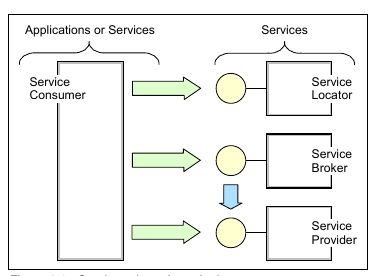
\includegraphics[width=0.80\textwidth]{img/7.png}
\caption{Plan de trabajo estándar del Conceptos esenciales de la Arquitectura Orientada a Servicios y la relación entre ellos
Fuente: Endrei et al. (2004)}
\label{figure:SOAworkflow}
\end{figure}

\section{Herramientas de software a utilizar}

Para la implementación del sistema se hizo uso de las siguientes herramientas de desarrollo web. Para la capa de interfaces de la aplicación, se utilizó Vue,js, un marco de trabajo desarrollado en JavaScript, que integra el etiquetado estándar de la web, así como soporte para estilos personalizados y lógica funcional. Por otra parte, del lado de la capa de datos, se desarrolló sobre Feathers.js, un marco de trabajo desarrollado enteramente en JavaScript que corre sobre el entorno de ejecución Node.js, que se comunica con una base de datos no relacional orientada a documentos MongoDB, mediante un mapeo objeto-documento a través de Mongoose. Finalmente, el lado del servidor fue desplegado en un entorno en la nube de Amazon Web Services, así como su entorno de desarrollo se encuentra alojado en MongoDB Atlas. A continuación, se mostrará a detalle cada herramienta utilizada para el desarrollo del producto final.

\subsection{Vue.js}

Vue (pronunciado /vjuː/, como view) \ref{figure:VueLogo} es un entorno de trabajo progresivo para desarrollar interfaces de usuario. Extraído de la página oficial del producto, ellos se describen a sí mismos de esta manera: “A diferencia de otros frameworks monolíticos, Vue está diseñado desde cero para ser utilizado incrementalmente. La librería central está enfocada solo en la capa de visualización, y es fácil de utilizar e integrar con otras librerías o proyectos existentes. Por otro lado, Vue también es perfectamente capaz de impulsar sofisticadas Single-Page Applications cuando se utiliza en combinación con herramientas modernas y librerías de apoyo”\cite{vuejs}.

\begin{figure}[H]
\centering
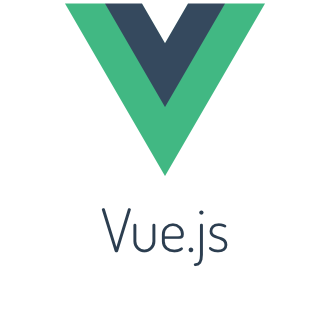
\includegraphics[width=0.80\textwidth]{img/8.png}
\caption{Logotipo de Vue.js
Fuente: https://vuejs.org/images/logo.png
Feathers}
\label{figure:VueLogo}
\end{figure}

\subsection{FeathersJS}

FeathersJS es un entorno de trabajo ligero utilizado para generar aplicaciones web de timepo real y APIs REST haciendo uso de JavaScript y TypeScript. Feathers en su núcleo es un conjunto de herramientas  que siguen una Arquitectura Orientada a Servicios, que permite construir prototipos y aplicaciones listas para ser desplegadas de manera rápida.

\begin{figure}[H]
\centering
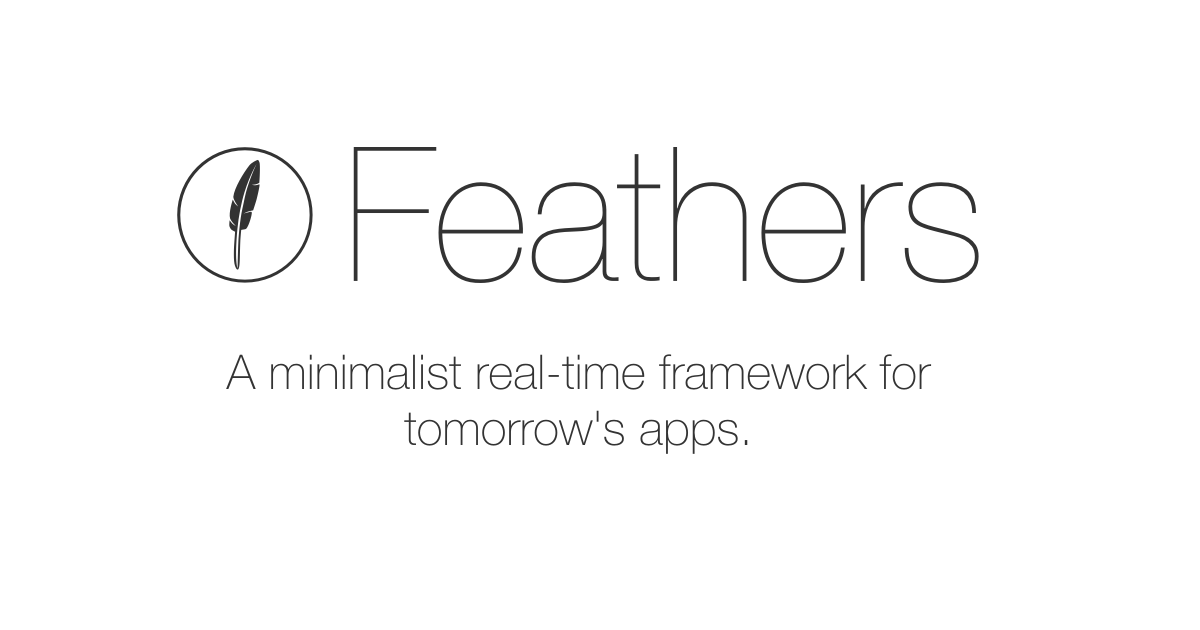
\includegraphics[width=0.80\textwidth]{img/9.png}
\caption{Logotipo de Feathers.js
Fuente: https://feathersjs.com/img/feathers-logo-wide.png}
\label{figure:FeathersLogo}
\end{figure}

De manera general, una aplicación construida en Feathers se puede dividir en tres secciones: el lado del cliente (NodeJS) que representa el espacio de conexión de Feathers como una API, el lado del servidor que maneja los datos y la lógica de negocios, y el núcleo funcional, que es utilizado tanto en el cliente como en el servidor.

\subsection{MongoDB}

MongoDB \cite{mongodb} es un sistema de base de datos multiplataforma de esquema libre orientado a documentos que ofrece una gran escalabilidad y flexibilidad, así como un modelo de consultas e indexación avanzado. Dentro de sus conceptos elementales, están los siguientes:

\begin{description}
    \item[Base de datos:] Una base de datos es un contenedor físico para colecciones.
    \item[Colección:] Una colección es un grupo de documentos de MongoDB. Es el equivalente a una tabla en una base de datos relacional. Una colección existe en una base de datos individual. Las colecciones no fuerzan la existencia de un esquema.
    \item[Documento:] Un documento es un conjunto de pares de clave-valor. Los documentos tienen esquemas dinámicos. Un esquema dinámico implica que los documentos en la misma colección no necesariamente deben tener el mismo conjunto de campos o estructura.
\end{description}

\begin{figure}[H]
\centering

\includegraphics[width=0.80\textwidth]{img/10.png}
\caption{Logotipo de MongoDB
Fuente: https://www.agiliacenter.com/wp-content/uploads/2017/04/mongo-db-logo.png}
\label{figure:MongoDBLogo}
\end{figure}


\subsection{MongoDB Atlas}

MongoDB Atlas es un servicio de almacenamiento de datos en la nube proveído por MongoDB que permite alojar bases de datos no relacionales orientadas a documentos gestionados por MongoDB que pueden ser utilizadas por distintas aplicaciones web. Es reconocido por su flexibilidad y escalabilidad, así como por su tracción entre grandes compañías (7-Eleven, SEGA, Telefónica),  sus protocolos integrados de seguridad y el diseño particular orientado a aumentar la productividad de los desarrolladores \cite{mongodbAtlas}.

\subsection{AWS}

Amazon Web Services, también conocida como AWS, es un conjunto de herramientas y servicios de computación en la nube de Amazon. Este servicio se lanzó oficialmente en 2006 y para junio de 2007 AWS ya contaba con una base de usuarios de aproximadamente 180 mil personas. Entre las empresas que la utilizan se encuentran algunas como Reddit, Foursquare, Pinterest, Netflix, la NASA o la CIA.

\begin{figure}[H]
\centering

\includegraphics[width=0.80\textwidth]{img/11.png}
\caption{Logotipo de Amazon Web Services
Fuente: https://upload.wikimedia.org/wikipedia/commons/thumb/9/93/Amazon_Web_Services_Logo.svg/1200px-Amazon_Web_Services_Logo.svg.png}
\label{figure:AwsLogo}
\end{figure}


\subsection{Vercel}

Vercel es una plataforma en la nube para sitios estáticos y funciones sin servidor que se adapta perfectamente a su flujo de trabajo. Permite a los desarrolladores alojar sitios web y servicios web que se implementan instantáneamente, escalan automáticamente y no requieren supervisión, todo sin configuración \cite{vercel}.






\section{Infraestructura Propuesta}

La infraestructura a nivel de las herramientas propuestas en el esquema previo fue la explicada en la Figura \ref{figure:infraDiagram}.

\begin{figure}[H]
\centering
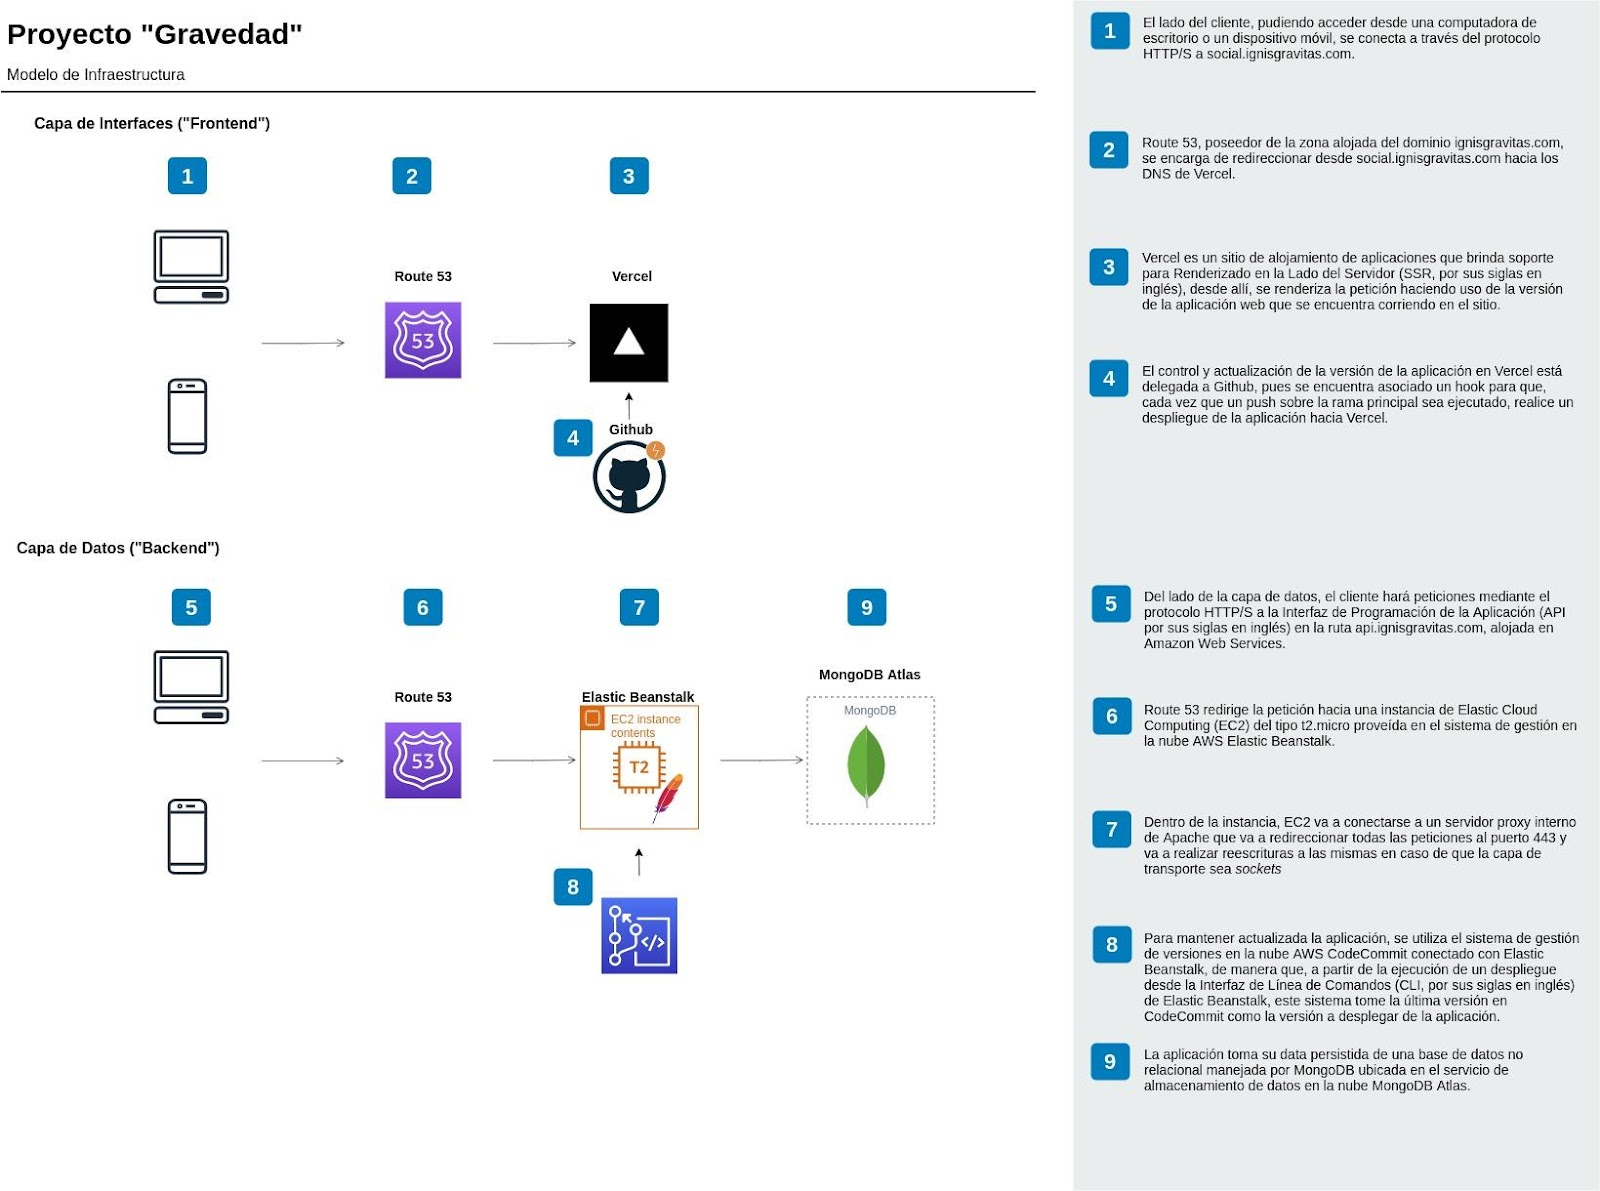
\includegraphics[width=0.80\textwidth]{img/13.jpg}
\caption{Infraestructura de capas del Proyecto “Gravedad”.
Fuente: Propia}
\label{figure:infraDiagram}
\end{figure}

Cada punto describe un elemento esencial dentro del sistema de funcionamiento de la aplicación.

    \begin{enumerate}
        \item El lado del cliente, pudiendo acceder desde una computadora de escritorio o un dispositivo móvil, se conecta a través del protocolo HTTP/S a \texttt{social.ignisgravitas.com}.
        \item Route 53, poseedor de la zona alojada del dominio ignisgravitas.com, se encarga de redireccionar desde \texttt{social.ignisgravitas.com} hacia los DNS de Vercel.
        \item Vercel es un sitio de alojamiento de aplicaciones que brinda soporte para Renderizado en la Lado del Servidor (SSR, por sus siglas en inglés), desde allí, se renderiza la petición haciendo uso de la versión de la aplicación web que se encuentra corriendo en el sitio.
        \item El control y actualización de la versión de la aplicación en Vercel está delegada a Github, pues se encuentra asociado un hook para que, cada vez que un push sobre la rama principal sea ejecutado, realice un despliegue de la aplicación hacia Vercel.
        \item Del lado de la capa de datos, el cliente hará peticiones mediante el protocolo HTTP/S a la Interfaz de Programación de la Aplicación (API por sus siglas en inglés) en la ruta \textt{api.ignisgravitas.com}, alojada en Amazon Web Services.
        \item Route 53 redirige la petición hacia una instancia de Elastic Cloud Computing (EC2) del tipo t2.micro proveída en el sistema de gestión en la nube AWS Elastic Beanstalk.
        \item Dentro de la instancia, EC2 va a conectarse a un servidor proxy interno de Apache que va a redireccionar todas las peticiones al puerto 443 y va a realizar reescrituras a las mismas en caso de que la capa de transporte sea sockets.
        \item Para mantener actualizada la aplicación, se utiliza el sistema de gestión de versiones en la nube AWS CodeCommit conectado con Elastic Beanstalk, de manera que, a partir de la ejecución de un despliegue desde la Interfaz de Línea de Comandos (CLI, por sus siglas en inglés) de Elastic Beanstalk, este sistema tome la última versión en CodeCommit como la versión a desplegar de la aplicación.
        \item La aplicación toma su data persistente de una base de datos no relacional manejada por MongoDB ubicada en el servicio de almacenamiento de datos en la nube MongoDB Atlas.
    \end{enumerate}